\documentclass{beamer}

% Preamble
\usepackage[utf8]{inputenc}
\usepackage{graphicx} 
\usepackage{amsmath} 
\usepackage{caption}
\usepackage{hyperref} 
\usepackage{xcolor} 
%\usepackage{fouriernc} %New Century Schoolbook with Fourier math

% Theme setup
\usetheme[secheader]{Madrid} 
\usecolortheme{beaver}

% Title page details
\title{Age from brain Data}
\subtitle{Project presentation}
\author{Marco Accerenzi}
\institute{Università di Pisa}
\institute[Università di Pisa]
{
  Dipartimento di Fisica
}
\date{\today}
\date[12 Settembre 2024] 
{Esame di Computing Methods for Exerimental Particle Physics and Data Analysis, 12 Settembre 2024}

\newcommand{\customSectionHeader}{
    \setbeamertemplate{section in head/foot}{}
    \setbeamertemplate{headline}{}
}



% Begin the document
\begin{document}

% Title Slide
{
    \customSectionHeader
	\begin{frame}
    	\titlepage
	\end{frame}
}

% Table of Contents
{
    \customSectionHeader
    \begin{frame}
        \title{Table of Contents}
        \tableofcontents
    \end{frame}
}

% First Slide--------------------------------------------------------------------------------------------------------------------------------------

\section{Introduzione}
\begin{frame}{Introduzione al progetto}
	L'obiettivo di questo progetto era sviluppare un modello di regressione di deep learning, addestrato per predire l'età cerebrale dei pazienti dai dati estratti dalla risonanza magnetica (MRI) dei loro cervelli.

Il modello implementato nel progetto è in grado di predire l'età dei pazienti nel set di dati con un errore quadratico medio (RMS) di circa 6 anni.

La configurazione migliore per il modello è stata un modello di deep learning con 2 hidden layers e 6 nodes per strato. Il modello si addestra e predice al meglio quando i dati sono standardizzati e normalizzati utilizzando i metodi forniti nel progetto.

\end{frame}


% Third Slide----------------------------------------------------------------------------------------------------------------------------------------------------

\subsection{Cosa c'è nel codice}
\begin{frame}{Cosa c'è nel codice}
Il codice sorgente di questo programma contiene diverse classi e alcuni script, al fine di fornire un framework per utilizzare i dati MRI in input dal file excel ``raw'' per produrre un modello addestrato in grado di fare previsioni, valutare e visualizzare tali previsioni.
\pause
    \begin{itemize}
		\item La classe ExcelData è responsabile della lettura del file excel e fornisce input adeguati per il modello.
\pause
		\item La classe RegressionModel contiene il modello stesso.
\pause
        \item I due script ``Console'' forniscono un'interfaccia utente di base.

        \item Lo script Optimizator permette di scegliere rapidamente i valori per gli iperparametri del modello.
\pause
		\item Lo script Analysis per l'analisi.
    \end{itemize}
\end{frame}


% Fifth Slide ----------------------------------------------------------------------------------------------------------------------------------------------------

\section{Estrazione e manipolazioni dei dati}
\subsection*{Estrazione dei dati}
\begin{frame}{Estrazione dei dati}
I dati della risonanza magnetica per l'addestramento del modello sono stati forniti per questo progetto sotto forma di due file .xlsx, contenenti le caratteristiche di 915 pazienti (o campioni). Per ogni campione, il file contiene anche il valore reale dell'età al momento della scansione (etichetta) e il nome del gruppo che ha fornito i dati per il campione (nome del gruppo).
\pause
\begin{itemize}
\item Utilizzando la funzione \emph{read\_excel} fornita dalla libreria \emph{Pandas}, la classe crea un dataframe che rappresenta i dati nel file di input, comprese le etichette delle colonne.
\pause
\item Il metodo \emph{to\_numpy} del dataframe viene poi utilizzato per estrarre i dati numerici da fornire al modello e viene mantenuto come proprietà dell'istanza ExcelData.
\end{itemize}
\pause
Tutte le manipolazioni sui dati vengono eseguite su copie dell'array \emph{numpy}.

I campioni possono essere mescolati prima dell'addestramento per prevenire l'overfitting, consentendo di produrre previsioni genuine sugli stessi dati di test e validazione utilizzati nell'addestramento.
\end{frame}


% Sixth Slide----------------------------------------------------------------------------------------------------------------------------------------------------

\subsection{Manipolazione dei dati}
\begin{frame}{Manipolazione dei dati}

I dati "grezzi" contengono diverse celle vuote e le varie caratteristiche hanno intervalli di valori molto differenti. Per affrontare questo problema, i dati vengono standardizzati e normalizzati.
\pause
\begin{itemize}
\item Durante la lettura del file excel, ogni cella vuota viene riempita con il valore -9999.
\pause
\item Tutte le colonne dell'array vengono normalizzate: ogni cella viene divisa per il valore massimo di ciascuna colonna. In questo calcolo, le celle contenenti il valore -9999 vengono escluse.
\pause
\item Il modello si allenerà per ignorare i valori -9999. Questo consente di utilizzare un set di dati più ampio rispetto a quello ottenuto eliminando tutti i campioni con una caratteristica mancante.
\pause
\item La normalizzazione e la standardizzazione riducono notevolmente il tempo necessario per l'addestramento. Le istanze del modello addestrate con dati normalizzati fanno previsioni mediamente più accurate sui dati rispetto a quelle addestrate senza normalizzazione.
\end{itemize}

\end{frame}


% Seventh Slide ----------------------------------------------------------------------------------------------------------------------------------------------------

\subsection{L'effetto della normalizzazione}
\begin{frame}{L'effetto della normalizzazione 1}
\centering
\begin{minipage}{0.48\textwidth}
	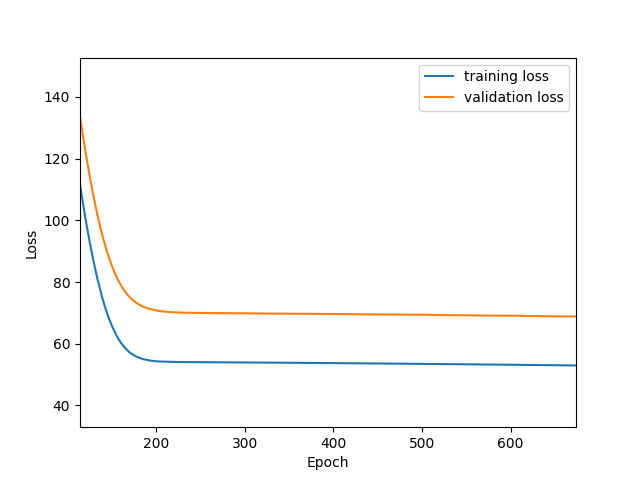
\includegraphics[width=\textwidth]{Figure_2.png}
	\captionof{figure}{Grafico delle prime epoche di addestramento utilizzando dati normalizzati.}
	\label{historyNormalised}
\end{minipage}
\begin{minipage}{0.48\textwidth}
	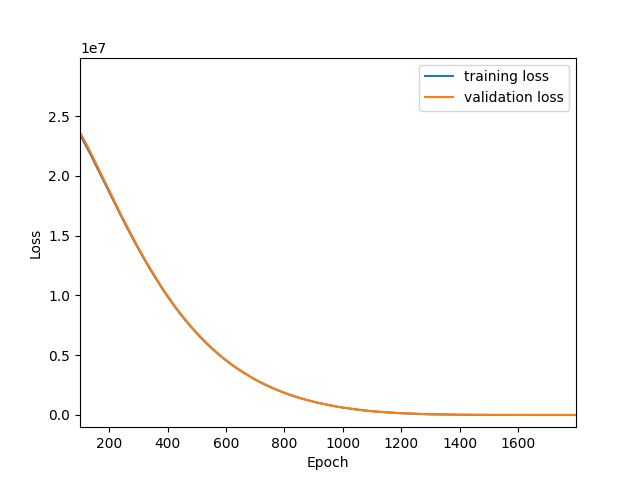
\includegraphics[width=\textwidth]{History_subplot_1.png}
	\captionof{figure}{Grafico delle prime epoche di addestramento utilizzando dati grezzi.}
	\label{historyNonNormalised}
\end{minipage}

\end{frame}




% Ninth Slide ----------------------------------------------------------------------------------------------------------------------------------------------------

\section{Il regression model}
\begin{frame}{Il regression model}
La classe del modello di regressione utilizza i moduli \emph{models}, \emph{layers} e \emph{callbacks} della libreria \emph{keras}.
Implementa diversi metodi:
\pause
\begin{itemize}
\item Il metodo Compile\_Model definisce l'istanza del modello, imposta i livelli e i nodi del modello e stabilisce la forma dei dati di input. Dopo la chiamata del metodo Compile\_Model, il modello viene compilato ed è pronto per l'addestramento.
\pause
\item Il metodo Start\_Training allena il modello su alcuni dati, utilizzando l'algoritmo di apprendimento supervisionato fornito dalla libreria \emph{keras}. Il numero di epoche e altri parametri dell'addestramento possono essere forniti dall'utente.
\pause
\item I metodi Plot\_History e Save\_Model sono pensati per essere utilizzati dopo Start\_Training, per salvare la cronologia dell'addestramento e il modello stesso.
\pause
\item Durante l'inizializzazione di un'istanza del modello è possibile utilizzare la funzione \emph{load\_model} per caricare un modello già addestrato: questo modello può essere utilizzato solo per l'inferenza e non per ulteriori addestramenti.
\end{itemize}

\end{frame}

% Tenth slide ----------------------------------------------------------------------------------------------------------------------------------------------------

\subsection{Callbacks}
\begin{frame}{Callbacks}
Per ottimizzare la fase di addestramento vengono utilizzati diversi callback:
\pause
    \begin{itemize}
        \item Early stopping:
			Questo callback interrompe l'addestramento se, dopo un numero di epoche successive impostato dall'utente, la funzione di perdita non è diminuita. Permette di fermare l'addestramento prima di incorrere in overfitting. Dopo l'interruzione, ripristina i pesi con le migliori prestazioni.
\pause        
\item ModelCheckpoint:
				Questo callback salva vari ``checkpoint'' durante l'addestramento. Permette di mantenere un backup del progresso dell'addestramento.
\pause        
\item ReduceLROnPlateau:
				Questo callback riduce il \emph{learning rate} del modello se l'addestramento raggiunge un plateau (significa se per un certo numero di epoche la funzione di perdita smette di diminuire). Riduce la quantità con cui i pesi del modello vengono cambiati durante l'addestramento, permettendo un ulteriore addestramento dopo aver raggiunto i plateaux.
\pause			
\item PrintProgress:
				Questa è una versione modificata di Callback della libreria \emph{keras}. Stampa le funzioni di perdita ogni n epoche. Il parametro n è impostato dall'utente attraverso un parametro ``verbose\_training'' del metodo Start\_Training.
    \end{itemize}
\end{frame}

% Thirteenth slide ----------------------------------------------------------------------------------------------------------------------------------------------------

\subsection{Confronto dei risultati}
\begin{frame}{Confronto dei risultati}

	Le prestazioni del modello sui diversi gruppi sono confrontate nella figura sottostante: 
l'errore di previsione per i dati dei gruppi ``Caltech'', ``MaxMun'' e ``SBL'' è nettamente superiore alla media.

	\begin{figure}
		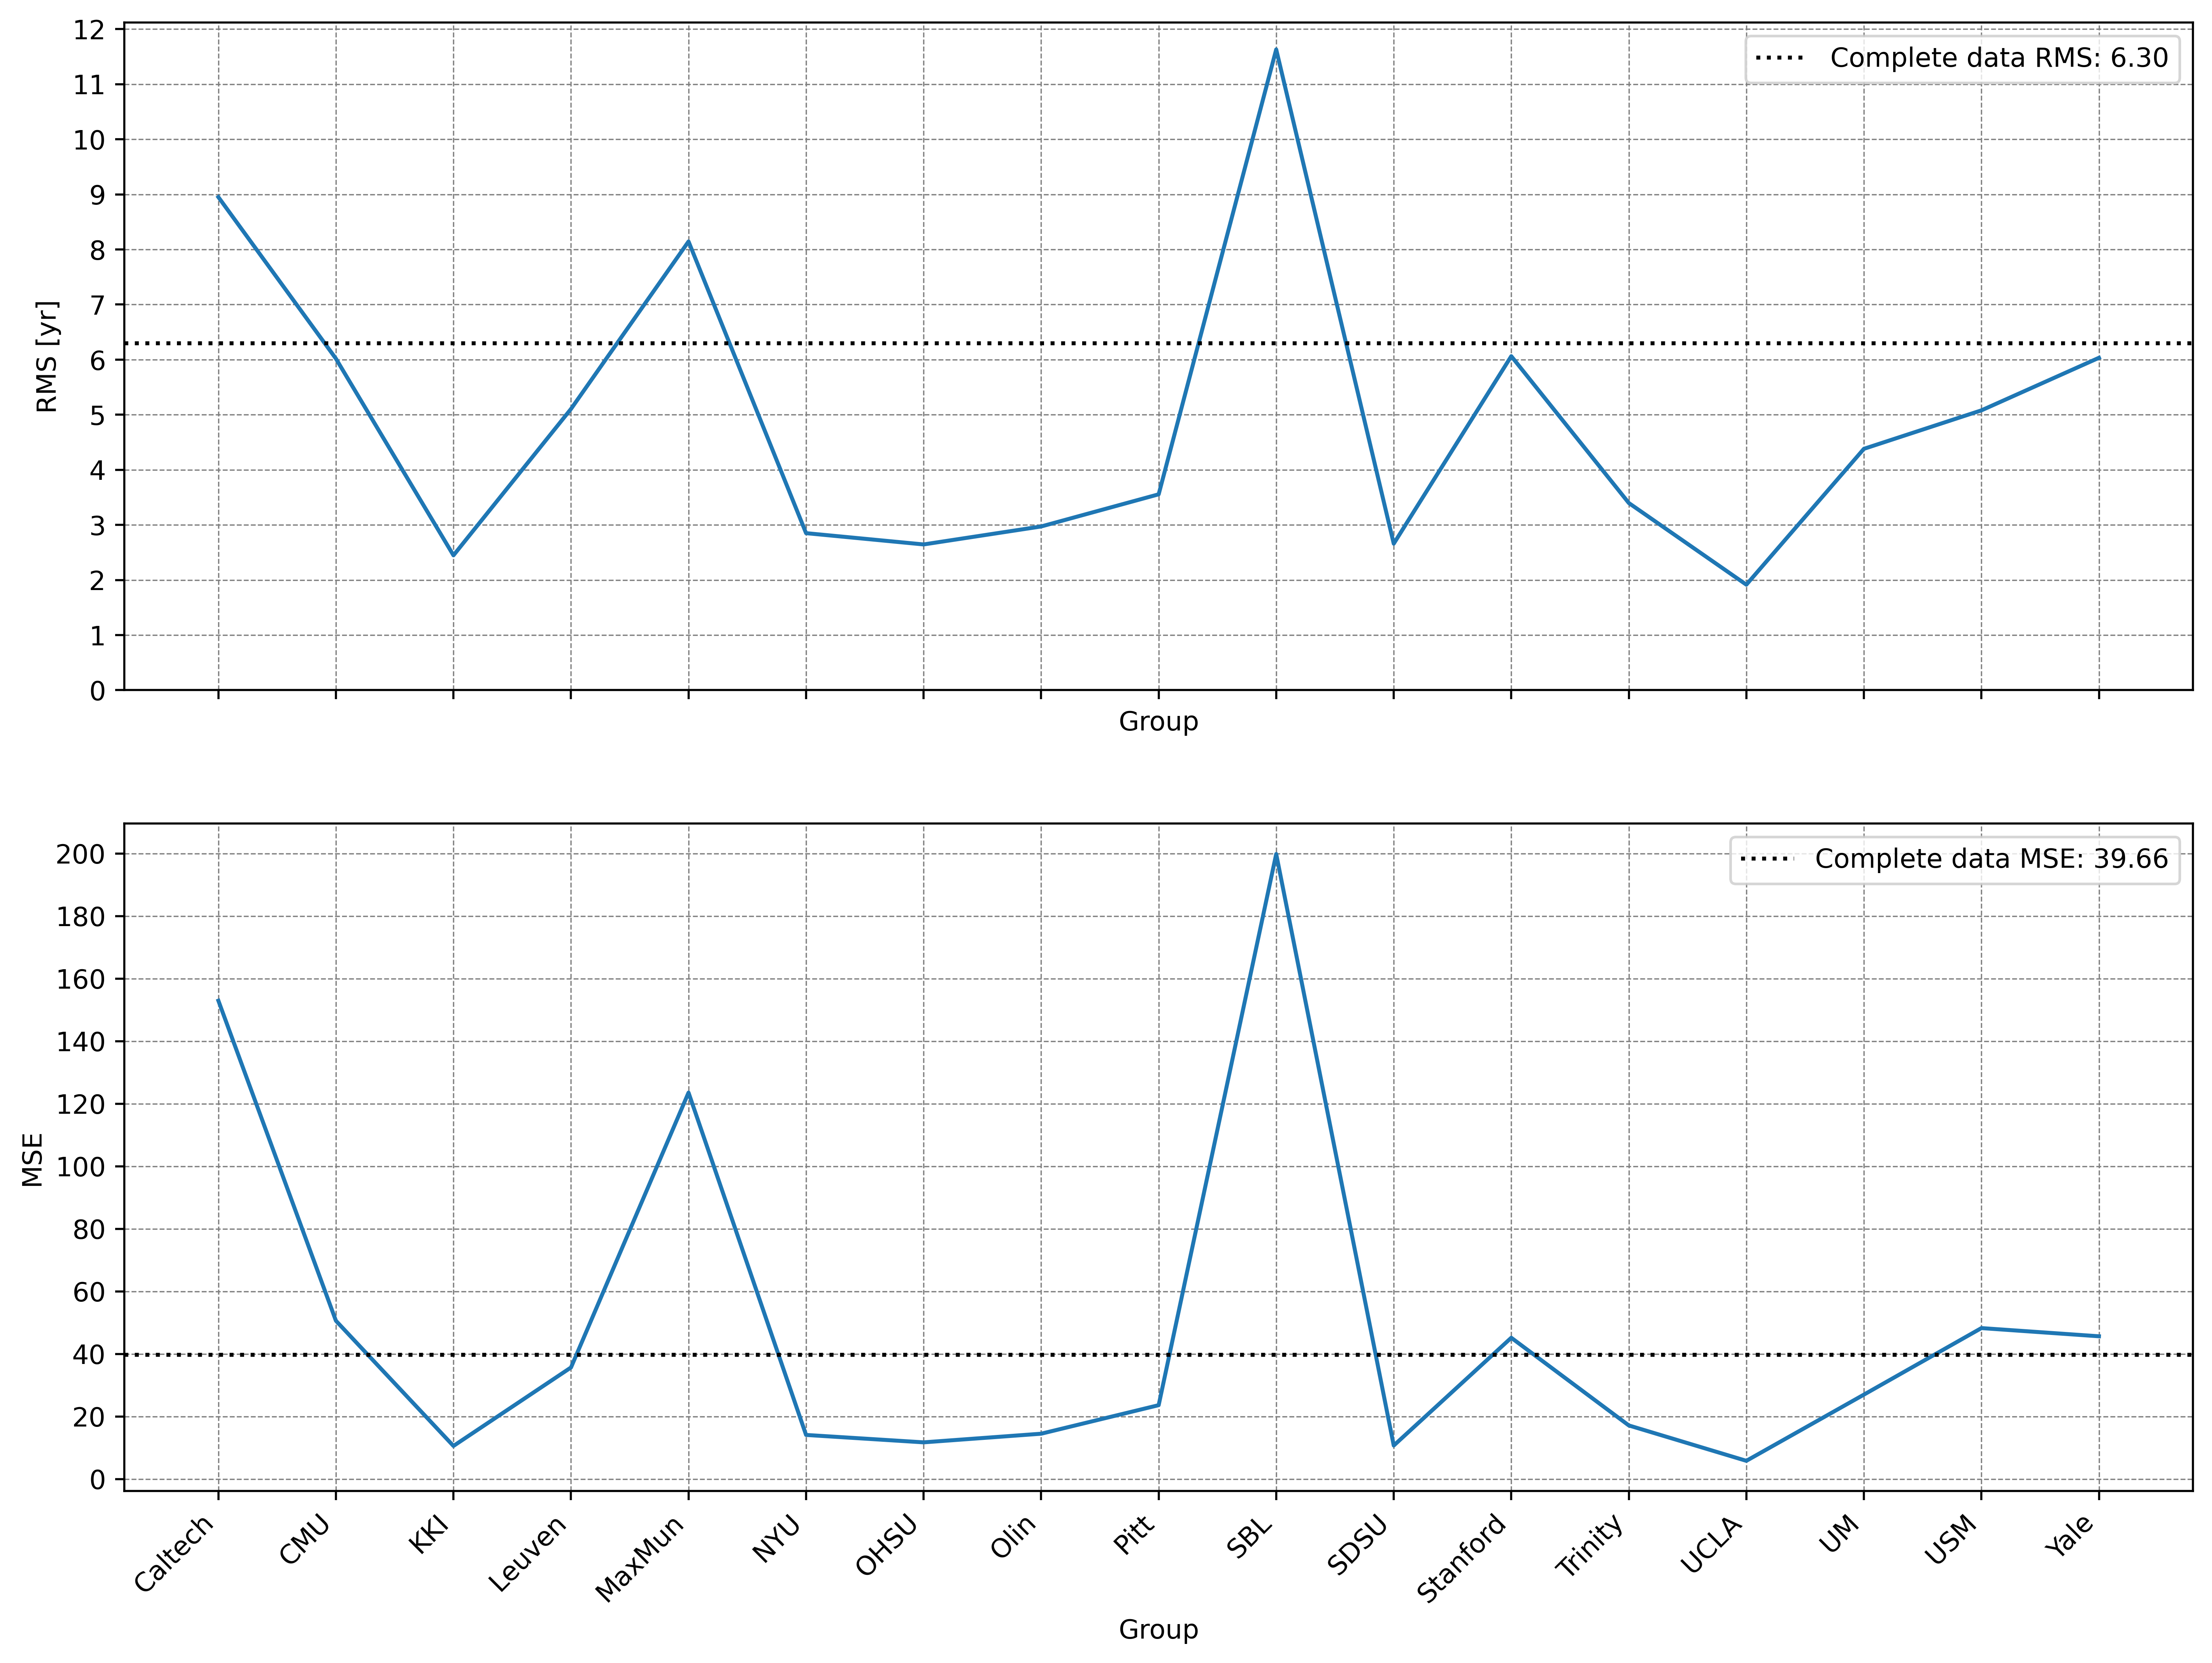
\includegraphics[width=0.65\textwidth]{result_1.png}
		\captionof{figure}{Grafico che confronta l'errore di previsione per i vari gruppi di dati. L'errore sull'intero set di dati è mostrato come una linea tratteggiata.}
		\label{plotRMSComparison2}
	\end{figure}

\end{frame}


%Fourteenth ----------------------------------------------------------------------------------------------------------------------------------------------------

\begin{frame}{Confronto dei risultati 2}

Ripetere l'addestramento su un set di dati ridotto, rimuovendo i tre gruppi di dati outlier, non migliora significativamente le prestazioni del modello: il modello addestrato si comporta in modo simile sui gruppi di dati rimanenti ma in modo significativamente peggiore per i tre outlier.

\begin{table}\centering
\begin{minipage}{0.45\textwidth}
	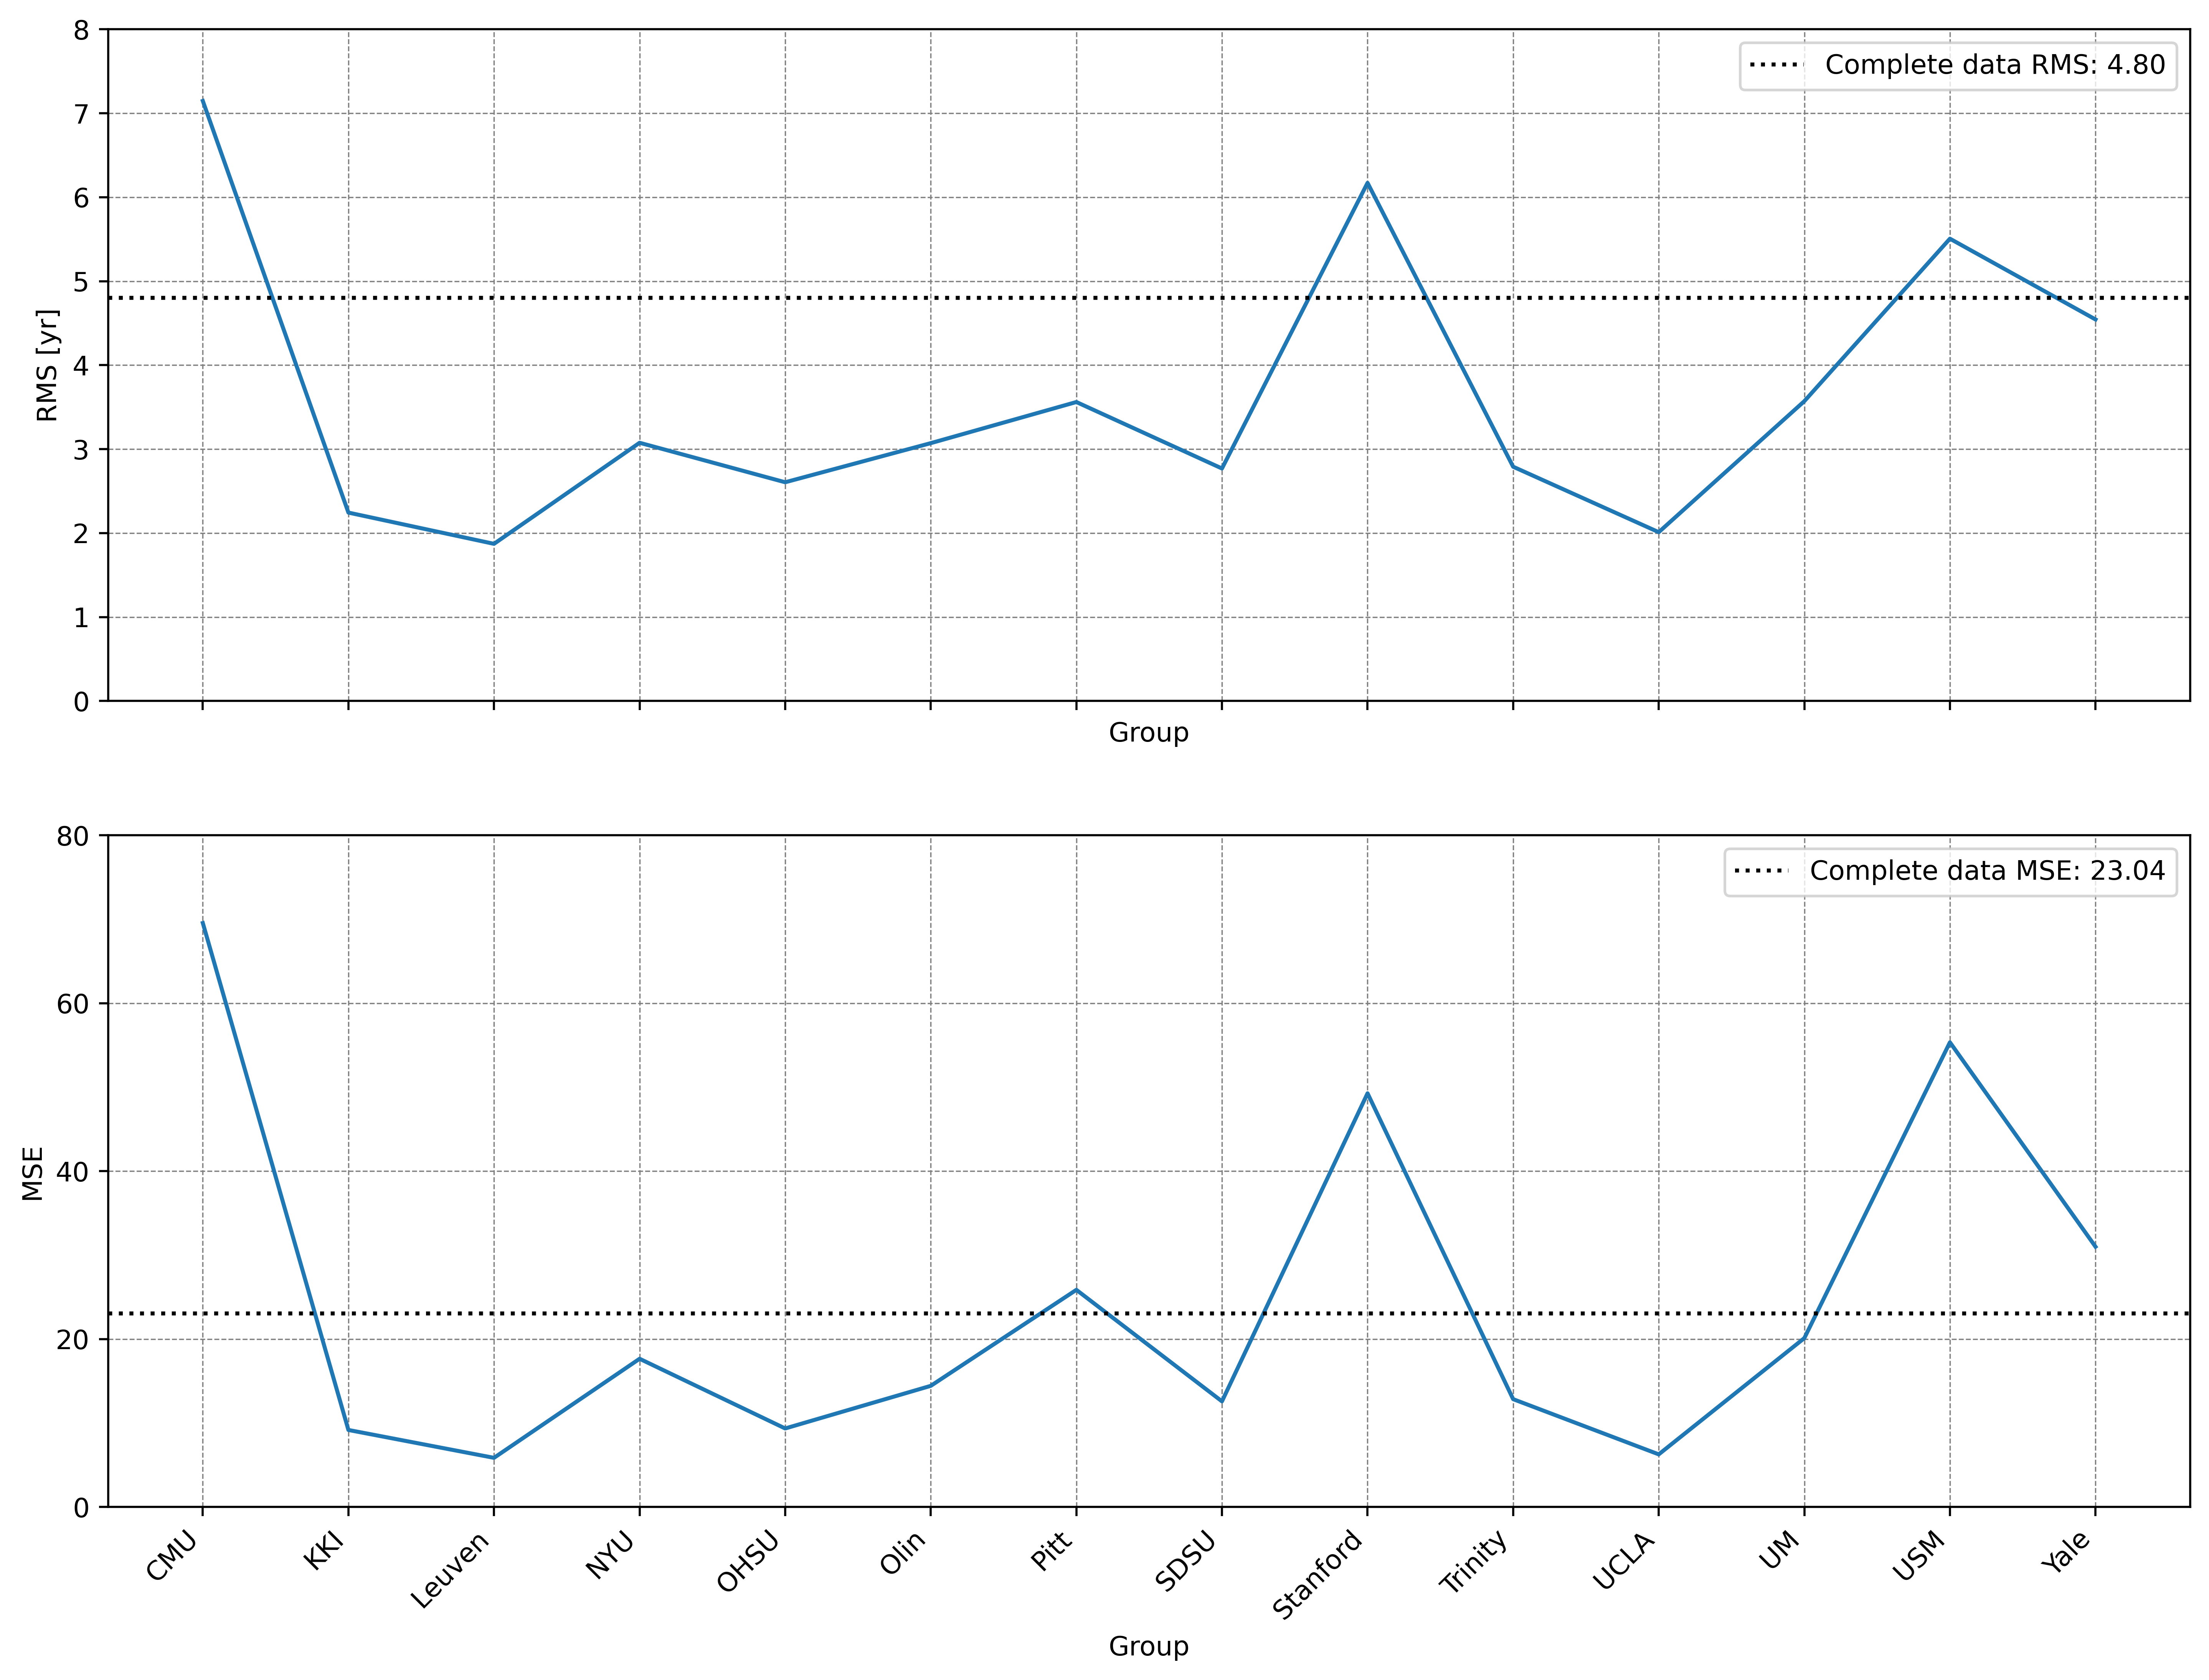
\includegraphics[width=\textwidth]{result_without_out.png}
\end{minipage}
\begin{minipage}{0.45\textwidth}
	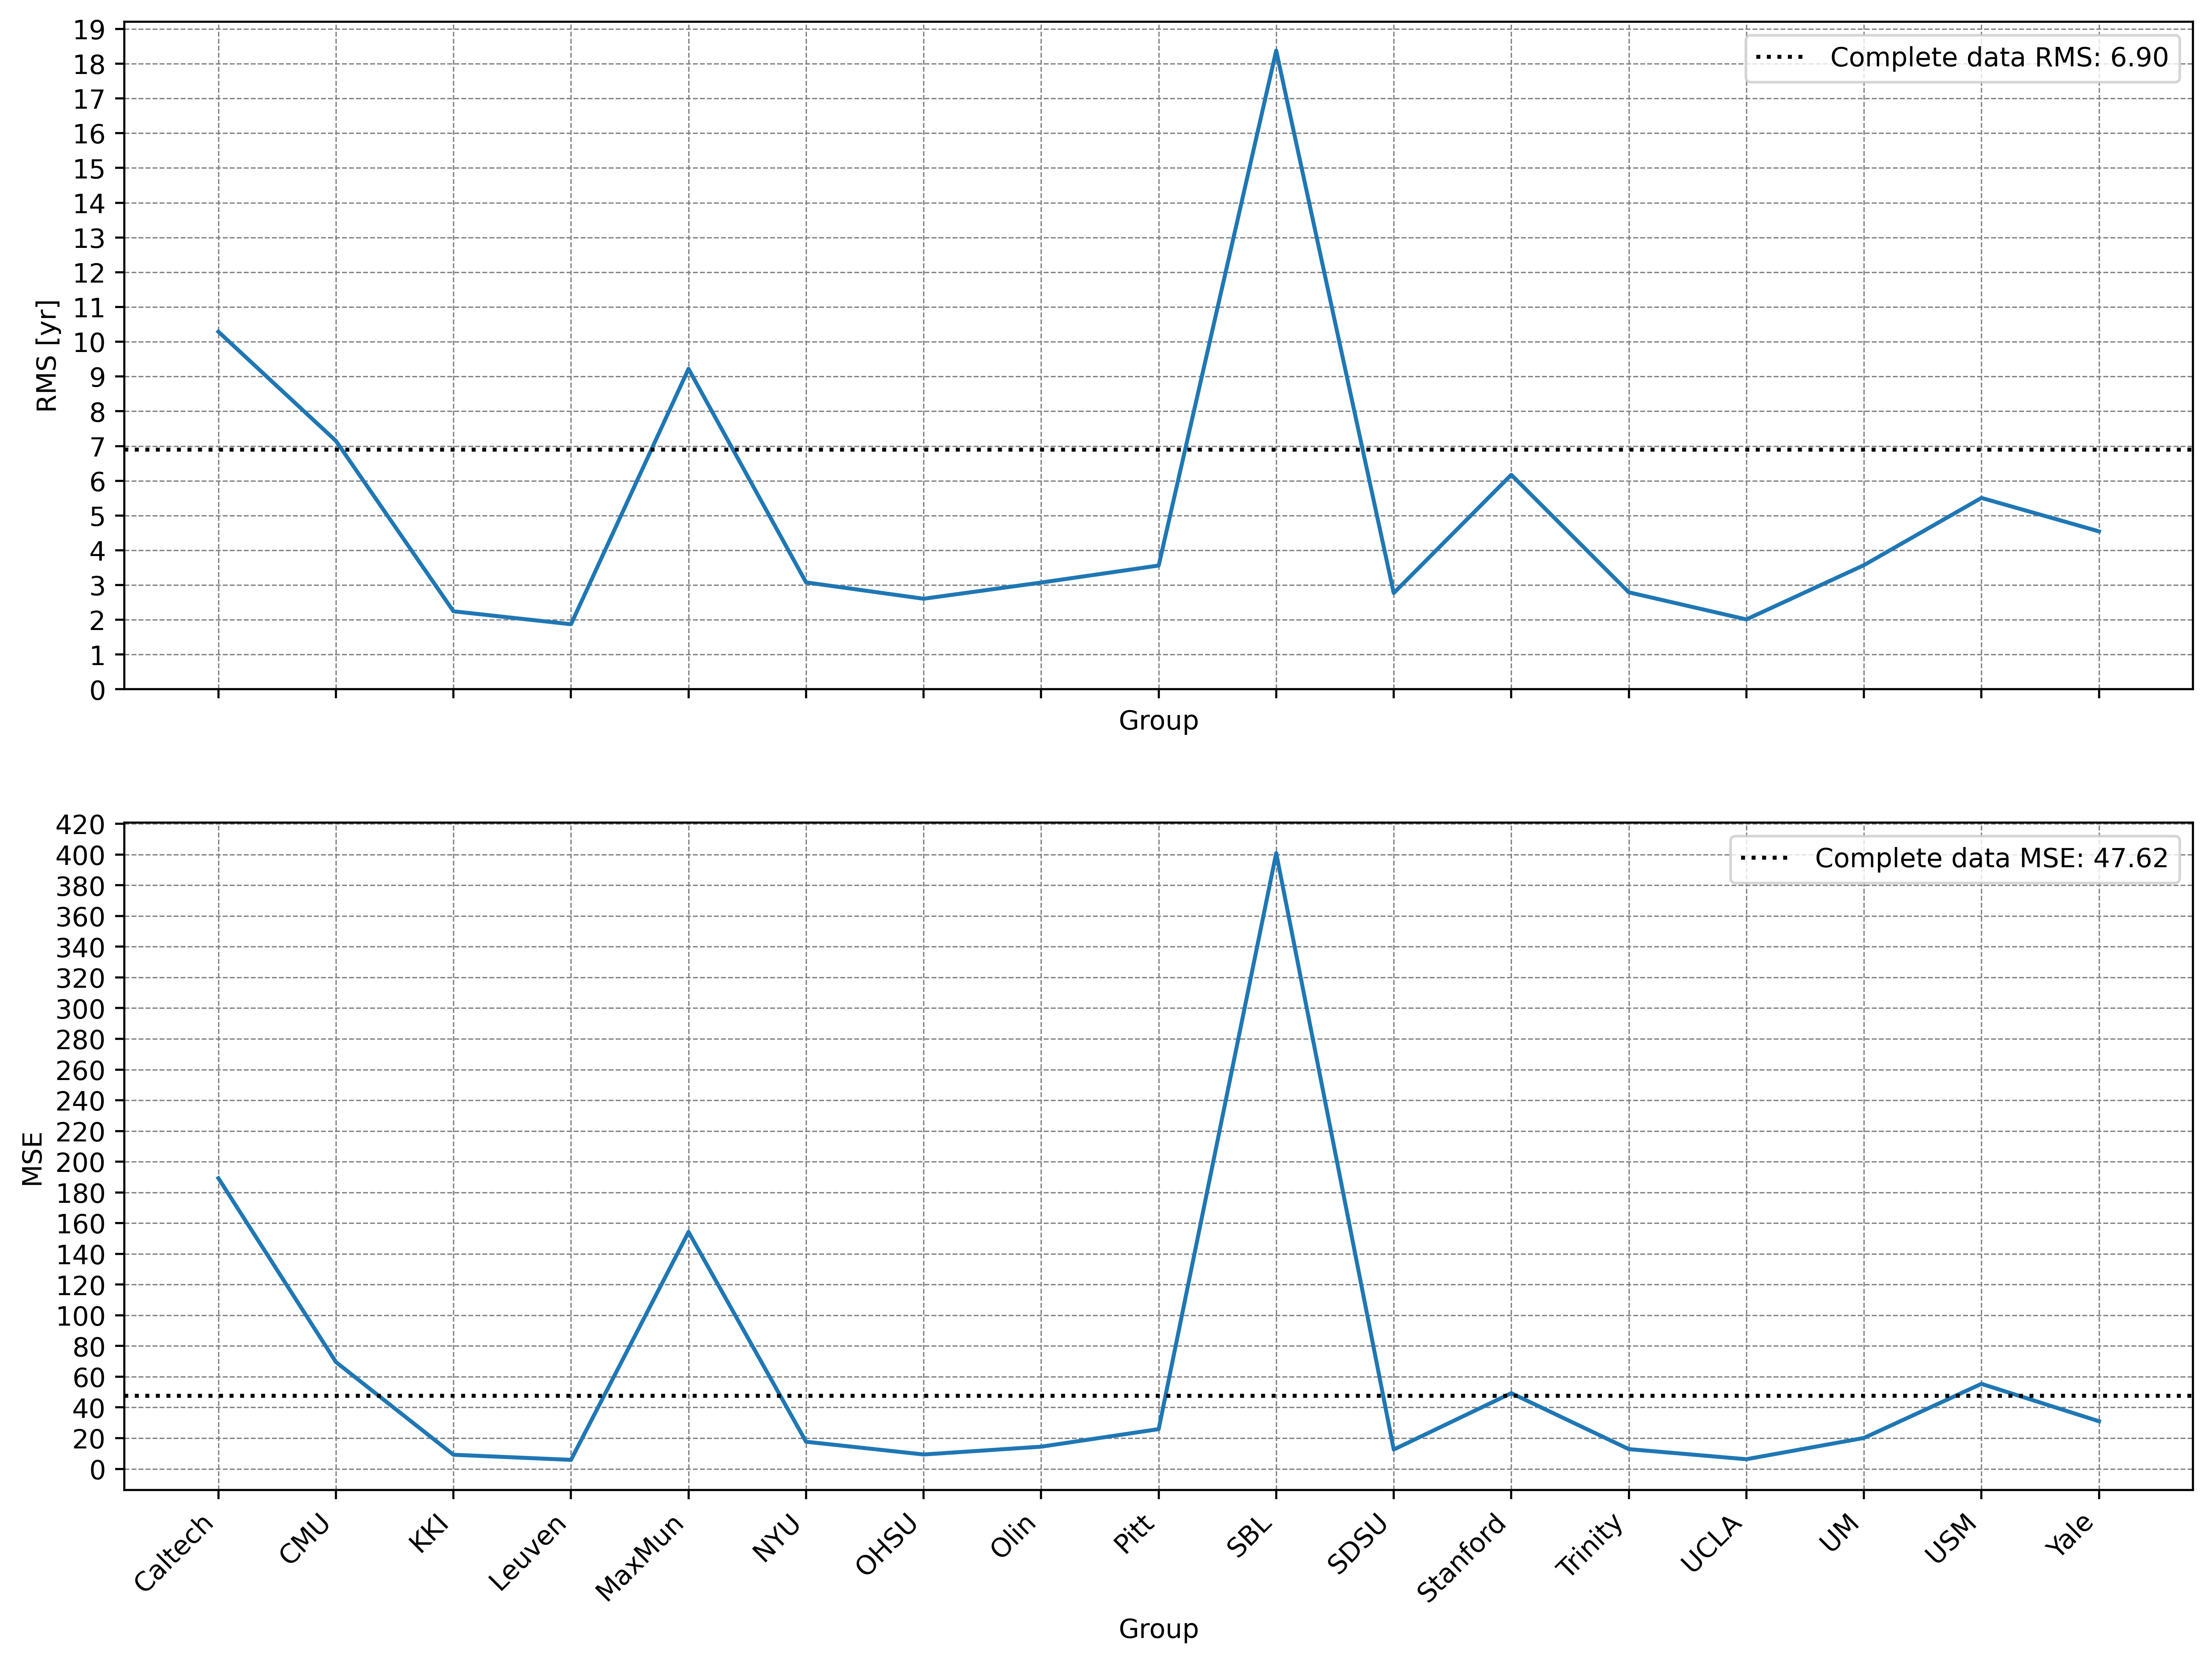
\includegraphics[width=\textwidth]{result_without_out_overall.png}
\end{minipage}
\end{table}

\end{frame}


%END ----------------------------------------------------------------------------------------------------------------------------------------------------

{
    \customSectionHeader
\begin{frame}
\centering
\Huge
\textbf{Grazie per l'attenzione!}
\end{frame}
}

% Backup slide 1 ----------------------------------------------------------------------------------------------------------------------------------------------------

\begin{frame}{Git e il repository}

Il progetto utilizza un repository pubblico su GitHub. 

Ha un ramo principale e tre rami attivi: develop, feature/docs e feature/presentation.

\end{frame}


% Backup slide 2 ----------------------------------------------------------------------------------------------------------------------------------------------------

\begin{frame}{Documentazione}

La documentazione del progetto è stata generata tramite Sphinx, utilizzando la sua funzionalità \emph{autodoc} per estrarre le docstring dal codice sorgente.

Il repository pubblico su GitHub consente di distribuire la documentazione del progetto attraverso ReadTheDocs e le Pages di GitHub.

\end{frame}





\end{document}
